\documentclass{article}

\usepackage{amsmath}
\usepackage{amssymb}
\usepackage[margin=1in]{geometry}
\usepackage{enumitem}
\usepackage{graphicx}
\graphicspath{{./}}

\title{Computer System Design Lab \# 7\\ISA Read}
\author{Amy Guo \\ Lab Partner: Charlie Coleman}
\date{April 30, 2018}

\newcommand{\Q}{\textbf{Q:}}
\newcommand{\A}{\textbf{A:}}
\newcommand{\sect}[1]{\noindent\textbf{#1}}

\begin{document}

\maketitle
\pagebreak

\sect{Pre-Lab:} Not applicable\\

\sect{Objective:} Design a VHDL design to drive an A/D converter (ADC) and record the output through the IO space via a C program written in DOS.\\

\sect{Circuit Diagram:} Not applicable\\

\sect{Outcome Predictions:} We will be able to record the ADC and reconstruct the signal that is output.\\

\sect{Equipment:}

\begin{itemize}[noitemsep, nolistsep]
	\item Xilinx Spartan 3 with MESA 4i38
	\item PC
	\item ADC0804
	\item Benchtop Power Supply
	\item Oscilloscope + Function Generator
\end{itemize}~

\sect{Procedure:}

\begin{enumerate}[noitemsep, nolistsep]
	\item Modify the VHDL design from Lab 6 to read 8 bit A-D conversions from IO pins.
	\item Write the A-D conversions to the IO space.
	\item Write a C script to fetch the A-D conversion from the IO space and print to the command line.
	\item Using the ADC0804 Spec sheet, assemble the circuit to allow for A-D conversion.
	\item Wire the 8 output pins of the ADC to the Spartan 3.
\end{enumerate}~

\sect{Recalculations and Predictions:} N.A\\

\sect{Data and Observations:}

\begin{center}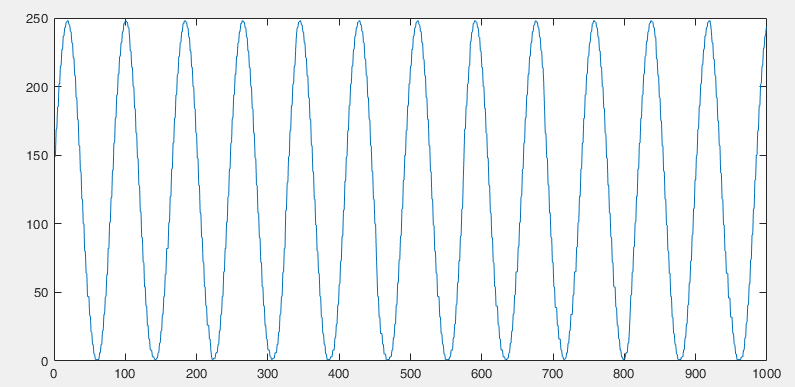
\includegraphics[width=\textwidth]{plot}\end{center}

We were able to obtain the graph above from our C program coupled with the Xilinx Spartan 3 + ADC0804. This graph matches our expectations exactly, as we were using the oscilloscope to generate a sine wave from 0 to 5, the full range of the ADC. \\

\sect{Analysis \& Discussion:} This lab was hard. We kept importing the wrong file because its name was too long, but after many hours we were able to find out we were importing the Lab 6 file. But then we imported the right file and everything began to work. We saw the expected values come out of the code.\\

\sect{Lab Questions:}

\begin{enumerate}[noitemsep,nolistsep]
	\item[\Q] What is the sample rate of your design?
	\item[\A] The maximum sample rate achieved by our design was 2000 samples/second.
	\item[\Q] What would be required to produce a variable sample rate design?
	\item[\A] The sample rate is determined by the clock rate of the VHDL design (set by the user) and the capacitor/resistor pair in the circuit. The clock rate could be reset during execution via some extra code, but to change the hardware sample rate would require a potentiometer in place of the resistor or some form of variable capacitance capacitor.
	\item[\Q] What voltage ranges can your design read?
	\item[\A] 0 to 5V
	\item[\Q] What changes would be required to be able to read wall voltage?
	\item[\A] The reference voltages would need to be 0-120V, but the ADC0804 is not capable of such high voltages. The chip would need to be replaced with something capable of high power operation.
\end{enumerate}~

\sect{Results:} This experiment worked as expected. The data output by our C program closely matched the expected range and waveform shape. \\

\sect{Conclusions:} In this lab, we learned how to assemble a circuit based off of data sheets. This is useful because many times we will not have a circuit that we are reproducing, but will simply be tasked with creating our own that matches given specifications and works with the given hardware. We also learned not to name our files anything longer than 8 characters as this will confuse DOS and lead to prolonged periods of debugging.

\end{document}
